\documentclass[aspectratio=169]{beamer}
\usepackage{basileabeam}

%notes
%\pgfpagesuselayout{2 on 1}[a4paper,border shrink=5mm]
%\setbeamertemplate{note page}[plain]
%\setbeameroption{show notes on second screen=bottom}

\title              {Title}

\author             {Author}
\email              {author@email.com}
\institute          {Institute, University of Basel}

\date               {Date}

\ulogo        		{Template/header}
\ulistelement    	{Template/listelement}

\graphicspath{{Figures/}}


\begin{document}
\begin{frame}[t,plain]
\titlepage
\end{frame}

\note{Notes can help you to remember important information. Turn on the notes option.}

\begin{frame}[c]{Some Images}
\begin{columns}[c]
    \column{.55\textwidth}
            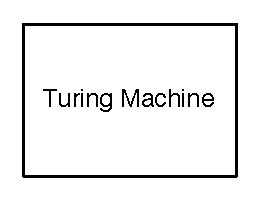
\includegraphics[width=0.8\textwidth]{block}
    \column{.45\textwidth}
            Turing machine
\end{columns}
\end{frame}

\note{Notes can help you to remember important information. Turn on the notes option.}

\begin{frame}[c]{Some Images}
    \begin{figure}
        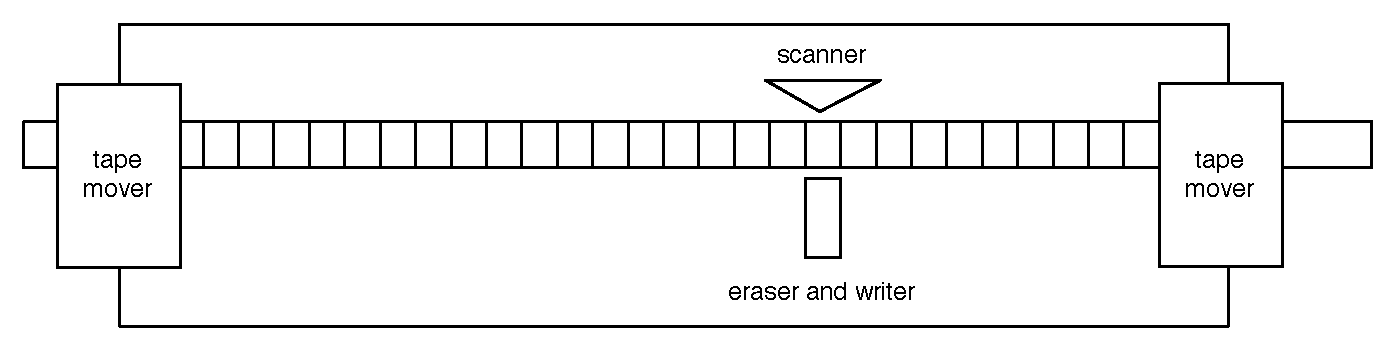
\includegraphics[width=0.8\textwidth]{turingmachine}
        \caption{A Turing Machine.}
    \end{figure}
\end{frame}

\note{Notes can help you to remember important information. Turn on the notes option.}

\begin{frame}[c]{Some Equations}
Now we introduce an equation.
\begin{theorem}
A Turing Machine is a 7-Tuple:
\begin{equation}
    M = \langle Q, \Gamma, b, \Sigma, \delta, q_0, F \rangle
\end{equation}
\end{theorem}
A Turing Machine is a 7-Tuple even if defined in the text, as in $M = \langle Q, \Gamma, b, \Sigma, \delta, q_0, F \rangle$.
\end{frame}

\note{Notes can help you to remember important information. Turn on the notes option.}

\begin{frame}[t]{Items and Numbers}
\begin{columns}
    \column{.5\textwidth}
            \begin{itemize}
            \item one
            \item two
            \item three
            \end{itemize}
    \column{.5\textwidth}
            \begin{enumerate}
            \item first
            \item second
            \item third
            \end{enumerate}
\end{columns}
\end{frame}


\note{Notes can help you to remember important information. Turn on the notes option.}

\begin{frame}[c]{Tables}
Tables are also interesting.
\begin{table}[ht!]
\centering
\begin{tabular}{|l|c|l|} \hline
Title&$f$&Comments\\ \hline
The chemical basis of morphogenesis & 7327 & \\ \hline
On computable numbers & 6347 & Turing Machine\\ \hline
Computing machinery and intelligence & 6130 & \\ \hline
\end{tabular}
\end{table}
\end{frame}

\note{Notes can help you to remember important information. Turn on the notes option.}

\begin{frame}[c]{Speaker Notes}
You may turn on the notes and handout option to see the notes to the slides.
\end{frame}

\note{Notes can help you to remember important information. Turn on the notes option.}

\begin{frame}[t,plain]
\lastpage{{\usebeamerfont{title} Questions?}\\[5ex]
author@email.com}
\end{frame}

\note{Notes can help you to remember important information. Turn on the notes option.}

\backupbegin

\begin{frame}{Backup}
Test
\end{frame}

\backupend

\end{document}

